Besides reaction wheels, one for each axis to be balanced around,  there are several other components. One motor to drive each reaction wheel and to control the motors an Arduino UNO R3\cite{arduino} was used. In addition, an Adafruit Motor Shield v2.0\cite{motorshield} was used to control the motors. The shield has the capability to distribute current to the motors of the system from the battery. Combined with Adafruit's library\cite{ms-lib}, the shield uses pulse-width modulation (PWM) to control speed and direction of DC motors. This was needed since it allows for a higher voltage and stronger current than what the Arduino can supply. The microcontroller reads the measurements from an inertial measurement unit (IMU) which calculates the current angle of the system. The IMU used was the BNO055 from Bosch Sensortec\cite{IMU-datasheet} with the help of Adafruit's library\cite{IMU-lib}.

\subsection{Single axis setup}
In order to get a better understanding of reaction wheel balancing a single axis setup was designed and 3D-printed. This setup can be seen in Figure~\ref{fig:SingleAxisV1}. The single axis setup was later modified and improved. The full assembly, including electronic components can be seen in figure \ref{fig:SingleAxisV2}. Despite it being a simple structure, it has the benefit of easy access to port. The microcontroller was not attached to the structure, it laid flat on the table. A prototype build like this allowed us to detect which components are sufficient for the end goal.

\begin{figure}
    \centering
    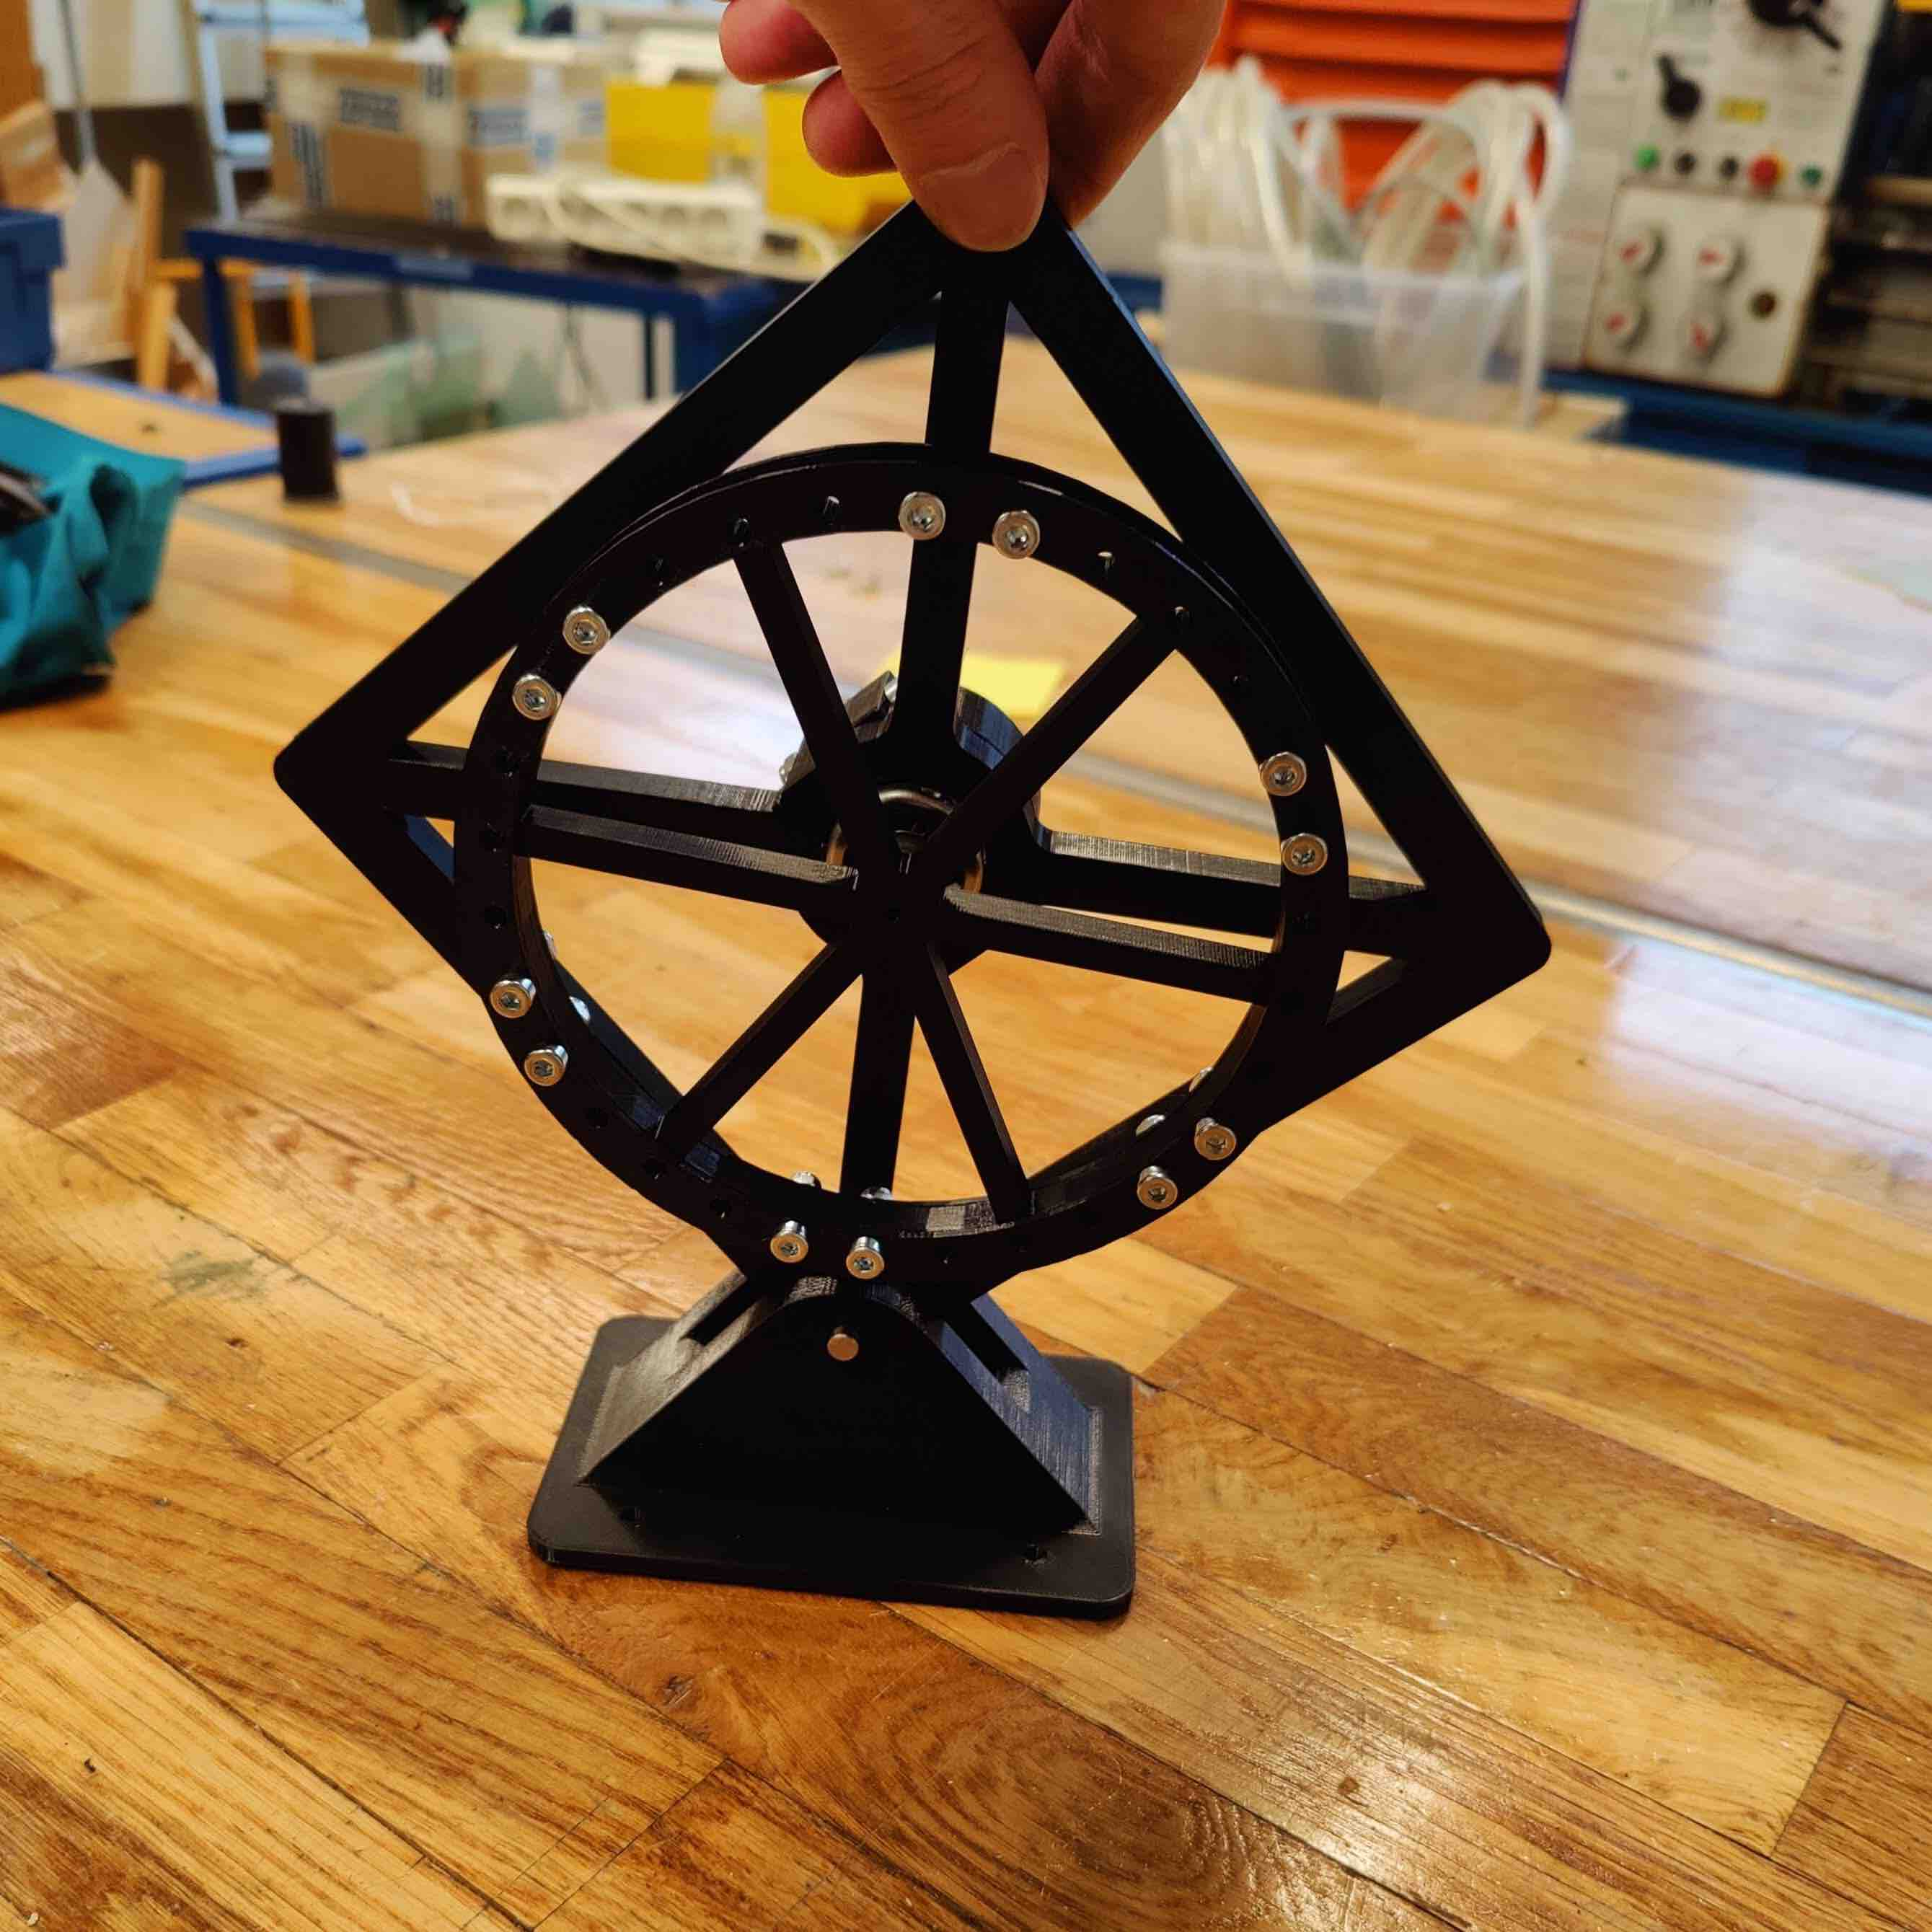
\includegraphics[width=0.6\linewidth]{figures/SingleAxisV1.jpg}
    \caption{The first version of the single axis setup}
    \label{fig:SingleAxisV1}
\end{figure}

\begin{figure}
    \centering
    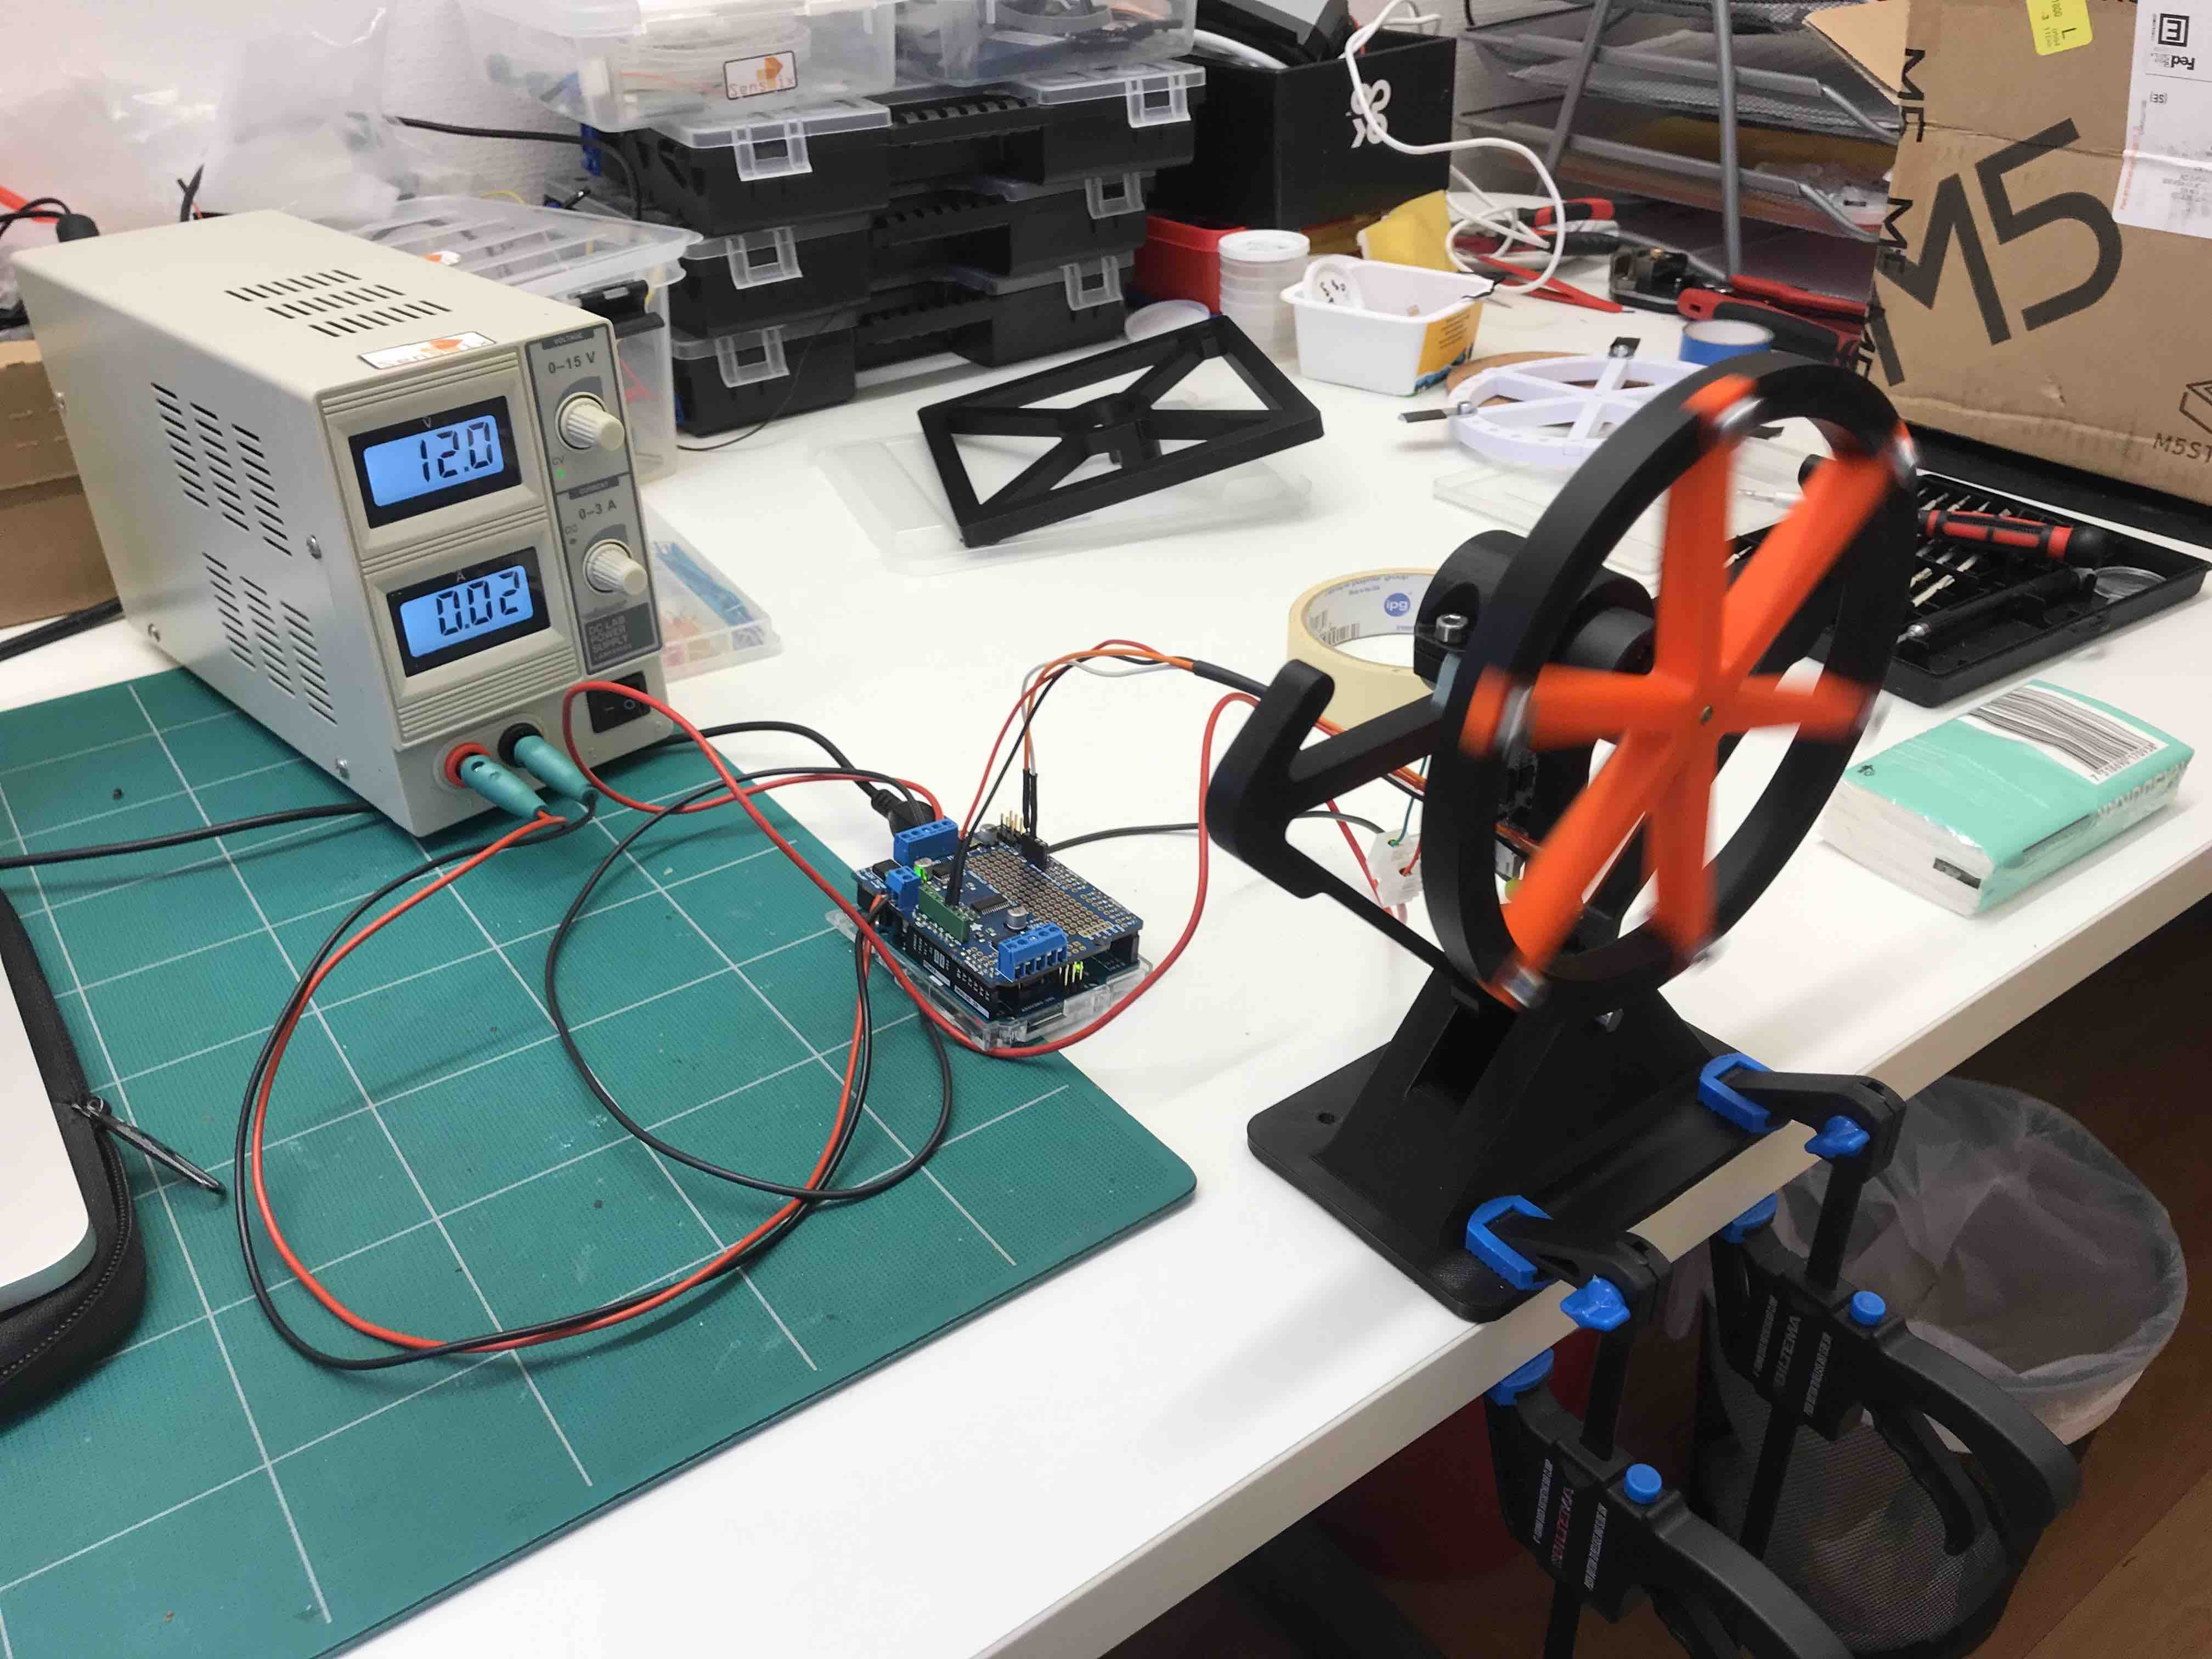
\includegraphics[width=.8\linewidth]{figures/SingleAxisV2Front.jpg}
    \caption{The second version of the single axis setup, with electrical components}
    \label{fig:SingleAxisV2}
\end{figure}

\subsection{The cube}
Designing the structure for the cube proved to be a lot more difficult and time consuming than expected. The intricate design demanded things to be decided based on assumptions, which later turned out to be incorrect. Some parts had to be redesigned multiple times. Some parts, e.g. four sides of the cube, were made identical to make the printing process less difficult. Other parts, engine mounts among them, were made symmetrical for the same reason. An advantage of having multiple identical parts is that if one part fails, it can potentially be replaced by another. While the replacement part is being printed, a side of the cube that is not critical when testing can be relocated into the critical position. The design of the cube can be seen in Figure~\ref{fig:cubediagram} with the parts named in Table~\ref{table:SystemComponents}.

%Här ska jonathans assembly bild in och referera till tabellen nedan.
\begin{figure}
    \centering
    \begin{subfigure}[h]{0.22\textwidth}
        \centering
        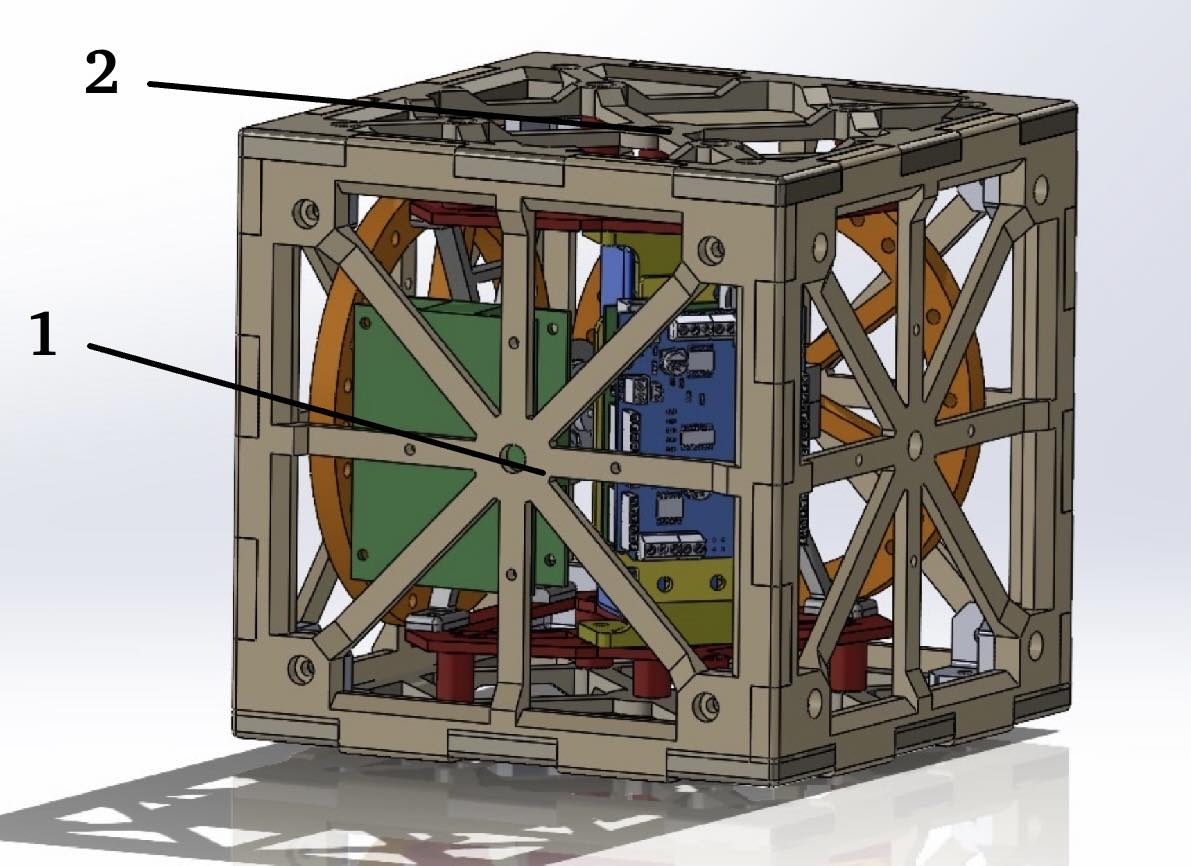
\includegraphics[width=\textwidth]{figures/Cube1.jpg}
    \end{subfigure}
    \begin{subfigure}[h]{0.22\textwidth}
        \centering
        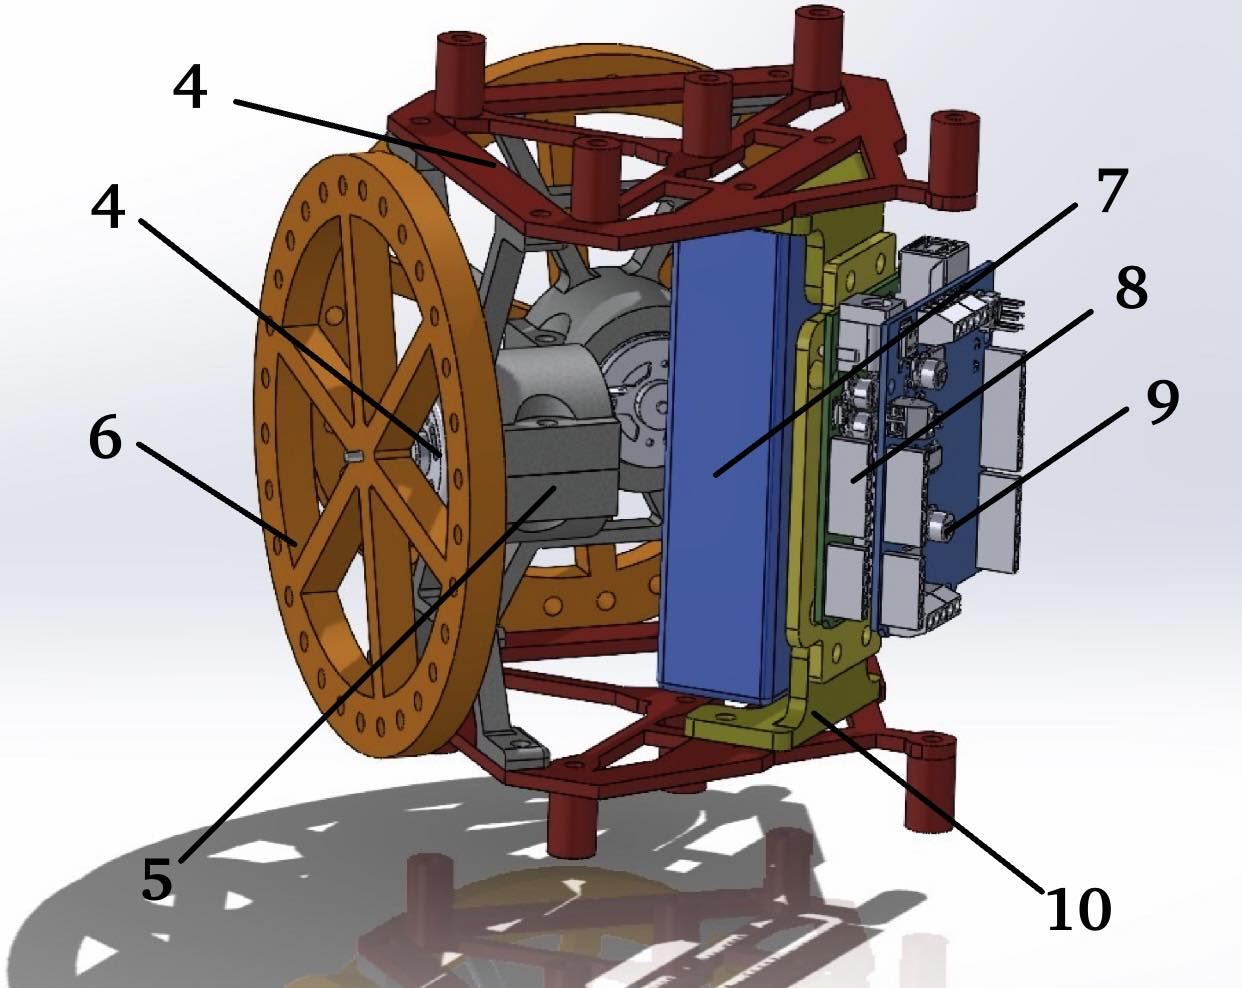
\includegraphics[width=\textwidth]{figures/cube2.jpg}
    \end{subfigure}
    \caption{The components in the system numbered.}
    \label{fig:cubediagram}
\end{figure}

\begin{table}
    \centering
    \begin{tabular}{cc}\toprule
     Component & Number \\\midrule
     Cube, side               & 1\\
     Cube, top and bottom     & 2\\
     Mounting plate           & 3\\
     DC motor                 & 4\\
     Motor holder             & 5\\
     Reaction wheel           & 6\\
     Battery                  & 7\\
     Arduino                  & 8\\
     Arduino Shield           & 9\\
     Electronics holder       & 10\\\bottomrule
    \end{tabular}
    \caption{The components in the system.}
    \label{table:SystemComponents}
\end{table}